% This is LLNCS.DEM the demonstration file of
% the LaTeX macro package from Springer-Verlag
% for Lecture Notes in Computer Science,
% version 2.4 for LaTeX2e as of 16. April 2010
%
\documentclass{llncs}
%
\usepackage{makeidx}  % allows for indexgeneration
\usepackage[UTF8]{inputenc}
\usepackage{soul}
\usepackage{graphicx}

\hyphenation{CYCLONE}

%
\begin{document}
\pagestyle{headings} 
\mainmatter              % start of the contributions

\title{An economical security architecture for multi-cloud application deployments\\ in federated environments}

\titlerunning{Federated, multi-cloud security architecture}  % abbreviated title (for running head)

\author{Mathias Slawik\inst{1} \and Begüm Ilke Zilci\inst{1} \and Axel Küpper\inst{1} \and\\ Yuri Demchenko\inst{2} \and Christophe Blanchet\inst{3}}

\authorrunning{Slawik, et al.}

\institute{Telekom Innovation Laboratories, Technische Universität Berlin\\Service-centric Networking\\\email{mathias.slawik|ilke.zilci|axel.kuepper@tu-berlin.de} \and
UvA Information \and
CNRS Information}

\maketitle              % typeset the title of the contribution

\begin{abstract}
Contemporary multi-cloud application deployments require increasingly complex security architectures, especially within federated environments. However, increased complexity often leads to higher efforts and raised costs for managing and securing those applications. This publication establishes an economical and comprehensive security architecture which is readily instantiable, pertinent to concrete users' requirements, and builds upon up-to-date protocols and software. We highlight its feasibility by applying the architecture within the CYCLONE innovation action, deploying federated Bioinformatics applications within a productive cloud environment. At last, we put special emphasis on the reduced management efforts to highlight the economic benefits of following our approach.
\end{abstract}

\section{Introduction}

There is widespread usage of cloud technologies within contemporary application deployments. Examples include using VMs and containers for componentization of applications, relying on highly scalable public cloud infrastructures, and embracing the immutable infrastructure paradigm to structure scalable cloud services, possibly deployed to multiple clouds. As the architecture of these applications becomes more complex, securing them also presents many new challenges that we address in this publication.

Our contribution was devised in the CYCLONE research project that focuses on two main characteristics of contemporary cloud applications: they are deployed on multiple clouds, e.g., for increased resiliency or reduced latency, and they use federated identities for authentication and authorization, e.g., academic and 3rd party identities, such as Google and Facebook. The security architecture addresses requirements in these areas and therefore proves quite useful to the users. The project deliverables\footnote{\url{http://www.cyclone-project.eu/deliverables.html}} are complementary to this publication as they contain more information about the security architecture (D4.1), the APIs and data formats (D4.3), as well as the Bioinformatics Use Case (D3.1).

In order to be economically feasible, we decided to strive for the following four main solution qualities for our security architecture:

\begin{itemize}
	\item \textbf{Relevant.} By analyzing representative requirements of concrete users we ensure that we create a relevant architecture for contemporary cloud environments.
	\item \textbf{Readily instantiable.} As we publish all components as open source\footnote{\url{https://github.com/cyclone-project/}}, our security architecture becomes almost instantly instantiable, saving efforts and costs on the side of our users.
	\item \textbf{Comprehensible.} Through this article and the CYCLONE deliverables we provide a large volume of comprehensible supporting material, making it easy to follow and adapt our ideas.
	\item \textbf{Mature.} We use established software as well as common protocols and libraries to create a stable and mature environment. This is further highlighted when we apply the architecture within the CYCLONE Bioinformatics Use Case and roll out security functionality in a production environment.
\end{itemize}

As a methodology we apply "Design Science in Information Systems Research" by Hevner et al. \cite{HMPR04} that also structures our presentation: first, in order to define the application area of our contribution we define the stakeholders and analyze their requirements in Section \ref{sec:requirements}. Afterwards, to ensure research rigor, we give a comprehensive overview about related works in Section \ref{sec:related-work}. Then, we describe the architecture in detail in Section \ref{sec:architecture} before evaluating it in Section \ref{sec:evaluation}. The evaluation also incorporates a discussion on the economical benefits. We conclude this publication by explicating the future extensions and open issues in Section \ref{sec:future} before summarizing it in Section \ref{sec:summary}.

\section{Stakeholders and Requirements}
\label{sec:requirements}

This section provides an overview about the involved stakeholders and concludes with an analysis of their requirements regarding the security architecture.

\subsection{Stakeholders}

In general, we consider three stakeholder groups: \textit{Cloud Infrastructure Providers}, \textit{Application Service Providers} (ASPs), as well as \textit{Cloud Application End-Users}. \textit{Cloud Infrastructure Providers} provide computing, storage, and networking resources so that \textit{Application Service Providers} can use them as a deployment target for their applications. \textit{Cloud Application End-Users} consume those applications, for example, to realize business value in diverse use cases.

\subsection{Requirements}

In the following, we describe the three main requirements that are most pertinent to our contribution:

\subsubsection{Requirement 1: Federated authentication and authorization.}

Federated identities are quite common in cloud environments. The most pertinent example for our work are academic identities, provided by the research institutions of academic end-users. They are used, for example, to authenticate users to online libraries of scientific publishers and also to allow them to access shared research infrastructures. Additionally, in both private and business settings, using Facebook or Google identities to access cloud applications is quite popular.

We see that all stakeholder groups require the use of federated identities: \textit{Cloud Infrastructure Providers} make the daily tasks of the ASP's DevOps easier by enabling them to reuse their preexisting identities to login to administrative interfaces. \textit{Application Service Providers} wish to enable their \textit{End-Users} to use the most practical - or most secure - identity in order make their applications more attractive to users. Especially when \textit{End-Users} are allowed to share application data access, relying on federated identities for authorization can provide more trust than, for example, creating separate username/password pairs.

\ul{To sum up, the security architecture has to provide functionalities to both authenticate as well as authorize federated user identities in a secure manner.}

\subsubsection{Requirement 2: Secure deployment of multi-cloud applications}

There are a lot of reasons why \textit{Application Service Providers} deploy their application components to multiple clouds. For example, distributing front end servers into data centers near the \textit{End-Users} lowers latency and can improve the perceived quality of the offering. Furthermore, cloud services become quite resilient against negative impacts if they not only depend on one single cloud provider.

\ul{The security architecture should therefore allow the deployment of applications in multiple clouds while still providing all of the required security properties.}

\subsubsection{Requirement 3: Unified logging for distributed systems}

We find many systems to be distributed extensively, e.g., the underlying cloud infrastructure is often distributed over multiple data centers in different world regions while cloud services are frequently distributed over multiple cloud offerings. Gathering diagnostic messages or performance metrics from all of these systems in a unified system is oftentimes challenging. When such functionality is not available, debugging these systems as well as providing an audit trail becomes a very tedious endevour.

\ul{Therefore, the security architecture should provide unified logging capabilities for highly distributed systems.}

\section{Related Work}
\label{sec:related-work}

After establishing the stakeholders and their requirements, we now give an overview about the work related to our contribution.

\subsection{Standards and Organizations}



OAuth, OpenID, OpenID Connect, SAML, EduGAIN, XACML

% SAML authentication requests are cryptographically signed, so that they can be validated by the Identity Providers based on public-key cryptography.

\subsection{Implementations}

Shibboleth IdP/SP, Keycloak, SimpleSAMLPHP, PAM, Moonshot, Nuv.la, OIDCACF, OIDCACF implementations \label{sec:oidcacfi}

\subsection{Methodologies}

OWASP security threat modeling, data flow modeling, risk assessment model

\section{Security Architecture}
\label{sec:architecture}

\begin{figure}
	\vspace*{-0.5cm}
	\centering
	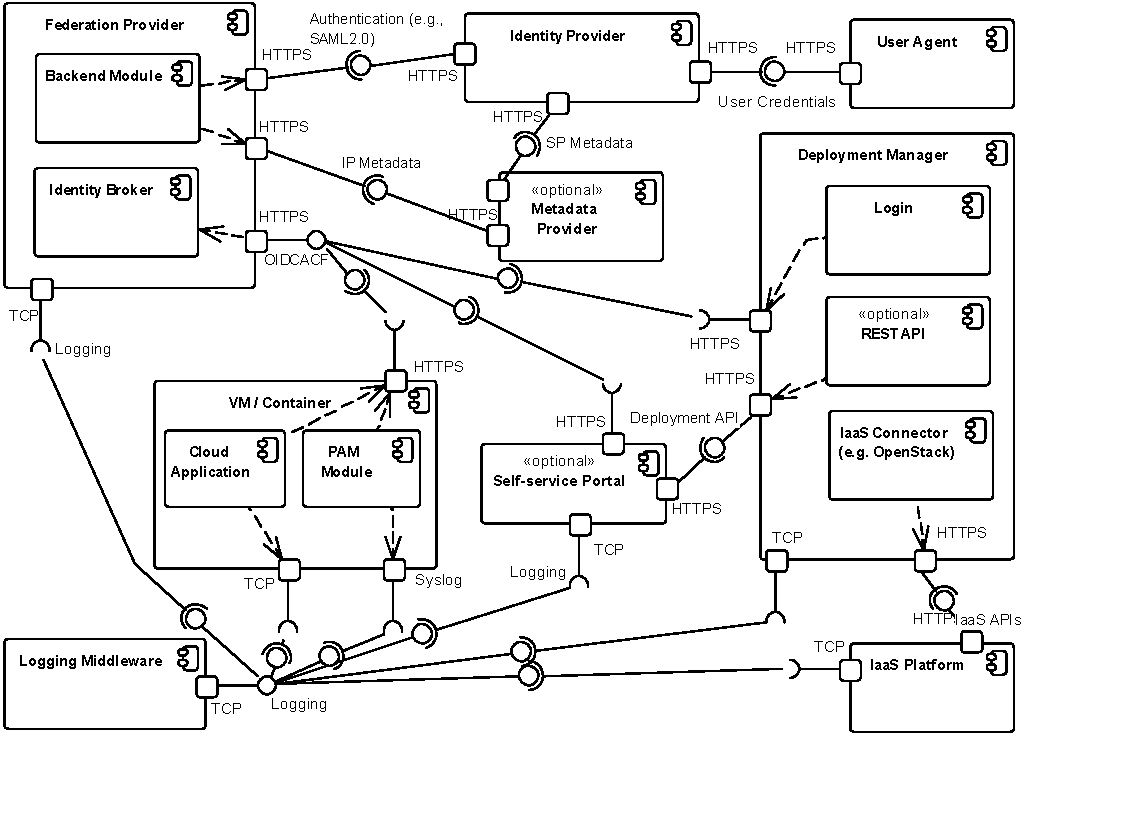
\includegraphics[width=\columnwidth, clip=true, trim=0cm 1.4cm 1.8cm 0cm]{uml_components}
	\caption{UML Component Diagram of the Security Architecture}
	\label{fig:architecture}
\end{figure}

Figure ~\ref{fig:architecture} shows the security architecture that we describe in this section. The following subsections explain its components in detail as well as how they implement the different security functions.

\subsection{Federation, Identity, and Metadata Provider}

On the top of the diagram there are three components related to federated authentication: The main component is the \textit{Federation Provider} that provides uniform user claims to relying applications, e.g., the user's identifier, their email addresses, and their home organization. These claims are contained within JSON web tokens retrieved using the OpenID Connect authentication code flow (OIDCACF). The \textit{Federation Provider} contains two subcomponents: first, the \textit{Identity Broker} where end-users can specify the identity they want to use for authentication, e.g., eduGAIN, Facebook, or a local Active Directory account. Second, the \textit{Backend Module} implementing the respective authentication protocol, e.g., SAML 2.0 or OpenID Connect.

The \textit{Federation Provider} communicates with different \textit{Identity Providers} that manage the accounts of the respective end-users, for example, it uses SAML 2.0 to communicate with the Shibboleth IdPs of the eduGAIN \textit{Identity Providers}. Both systems can use an optional \textit{Metadata Provider} (e.g., eduGAIN) to validate the signatures of the Federation Provider authentication requests by the Identity Providers.

The \textit{User Agents} of the end users transmit their local user credentials only to their respective Identity Providers. This provides both added security, as the credentials never leave the home domain of the users, as well as increased convenience, as end users can reuse their preexisting sessions to achieve web-based single sign-on. An example would be using the built-in Windows Authentication within an Active Directory-based environment.

As a side note: we refrain from calling the main component "Federated Identity Provider", as this leaves its role ambiguous: it can either be the same role (as in "provider of a federated identity") or it can be a regular \textit{Identity Provider} that is federated (as in "identity provider in a federation").

\subsection{Logging Middleware}

The main purpose of the logging middleware is providing network-accessible logging endpoints to unify log messages into a common format. These endpoints should comprise of at least a simple TCP-based and a syslog-compatible logger. The middleware is commonly complemented by two other systems not shown in the diagram, as they are not part of the core security architecture: a \textit{Logging Frontend}, allowing end-users to consume the logs, as well as a \textit{Logging Backend}, e.g., a database or flat files, to persist the logs.

\subsection{VM / Container}

Cloud applications are commonly deployed as virtual machines and/or in a container (e.g., Docker\footnote{\url{https://www.docker.com/}} or rkt\footnote{\url{https://github.com/coreos/rkt}}). These applications have three integration points with the security architecture: first, they rely on the OIDCACF to authenticate and authorize users - both on the application layer, through OpenID Connect libraries, as well as the OS layer, through the \textit{PAM module}. Second, they can log to the \textit{Logging Middleware}, e.g., through the simple TCP- as well as the syslog interface. Third, they rely on the \textit{Deployment Manager} to be deployed on the IaaS platform.

The \textit{PAM Module} allows the Linux operating system to authenticate users using their federated identities. In contrast to moonshot, it does not need a modified SSH client or server. Instead, it provides URLs to the users through the SSH "keyboard-interactive mode", which they open in their User Agents and carry out the regular OIDCACF. At the end, when the JSON web token is retrieved by the PAM module, it transforms the federated identities into existing or newly created local user accounts. More details can be found in the module source code\footnote{\url{add link}}.

\subsection{Deyploment Manager and Self-service Portal}

The \textit{Deployment Manager} provides many facilities to support multi-cloud application deployment, e.g., it can describe application topologies, connect to different IaaS platform APIs for multi-cloud deployment, and offers a web- and optionally a RESTful interface. It allows end-users to use the OIDCACF for logging in and it can write its log messages to the \textit{Logging Middleware}. While the architecture does not specify how the \textit{Deployment Manager} models applications internally, common deployment managers, such as Nuv.la, use modules to break down application components and use base images and deployment scripts as an internal application model.

There is another \textit{optional} component, the \textit{Self-service Portal}. It allows end-users without technical background to use the \textit{Deployment Manager} for instantiating VMs on the IaaS platform. Just like any other application, this Portal uses OIDCACF for authentication and authorization and logs to the network interfaces of the logging middleware. It communicates with the RESTful API of the \textit{Deployment Manager} in order to deploy and scale applications on preconfigured clouds.

\subsection{Security Functionality}

After specifying the components and their responsibilities we now describe how they interact to realize the main security functionalities \textit{application deployment}, \textit{federated authentication and authorization}, and \textit{distributed logging}.

\subsubsection{Application deployment}

The two-step application deployment process is described in the following, divided into \textit{preparing application modules} (Step 1) and \textit{multi-cloud application deployment and scaling} (Step 2):

\paragraph{Step 1: Preparing application modules.} As a first step, all application components need to be made deployable. This requires the preparation of instantiable \textit{deployment descriptions} containing all the steps necessary to create new instances of all application components. There are many different approaches to this, for example, Nuv.la allows the specification of a base image (e.g., "Ubuntu Linux LTS") and deployment scripts that are executed in order to install the respective application components on newly instantiated VMs. The deployments scripts also configure the components to use federated identities for authentication and authorization. This is described in detail in the following subsections.

\paragraph{Step 2: Multi-cloud application deployment and scaling.} After all application modules have been prepared, the \textit{Deployment Manager} uses the respective IaaS platform APIs to instantiate the base images as new VMs and runs the deployment scripts on them, either for initial deployment, or for subsequent scaling of the application. The same APIs are used to tear down the application when it is not needed anymore.

\subsubsection{Federated authentication and authorization}

In order to authenticate users based on their federated identities, cloud applications need to implement the OpenID Connect authentication code flow (OIDCACF). Using this workflow they can securely initiate authentication requests and retrieve claims about user identities from the \textit{Federation Provider}. When Application Service Providers prepare their application modules, they have different means of implementing the OIDCACF, as shown in section \ref{sec:oidcacfi}.

After authenticating users, cloud applications can use the cryptographically signed claims presented in the JSON Web Token for authorization. There is a set of attributes recommended for any eduGAIN identity provider that is shown in Table \ref{tab:eduGAIN-recommended-attributes}. The research institutions are free to implement any number of attributes and also additional attributes, for example group membership, in order to only allow certain users in this group access to the service. At last, the Federation Provider also supports creating local accounts or using a local LDAP for special cases not involving federated identities.

\def\arraystretch{1.5}
\begin{table}[]
	\centering
	\caption{eduGAIN recommended attributes}
	\label{tab:eduGAIN-recommended-attributes}
	\resizebox{\textwidth}{!}{%
		\begin{tabular}{|l|l|l|}
			\hline
			\textbf{Attribute} & \textbf{OID} & \textbf{Meaning} \\ \hline
			cn & 2.5.4.3 & Common name \\ \hline
			displayName & 2.16.840.1.113730.3.1.241 & Display name \\ \hline
			eduPersonAffiliation & 1.3.6.1.4.1.5923.1.1.1.1 & \begin{tabular}[c]{@{}l@{}}Users' affiliation\\ e.g., "staff", "student"\end{tabular} \\ \hline
			eduPersonScopedAffiliation & 1.3.6.1.4.1.5923.1.1.1.9 & \begin{tabular}[c]{@{}l@{}}Scoped affiliation\\ e.g., "staff@example.org"\end{tabular} \\ \hline
			mail & 0.9.2342.19200300.100.1.3 & Mail address \\ \hline
			schacHomeOrganization & 1.3.6.1.4.1.25178.1.2.9 & \begin{tabular}[c]{@{}l@{}}Home organization\\ e.g., "tu-berlin.de"\end{tabular} \\ \hline
			schacHomeOrganizationType & 1.3.6.1.4.1.25178.1.2.10 & \begin{tabular}[c]{@{}l@{}}Home organization type\\ e.g., university\end{tabular} \\ \hline
		\end{tabular}%
	}
\end{table}

\subsection{Distributed Logging}

As mentioned before, the \textit{Logging Middleware} should be quite flexible in the formats it accepts for logging as well as the structure of the log messages. For example, the Logstash middleware supports 49 different input plugins\footnote{See: \url{https://www.elastic.co/guide/en/logstash/current/input-plugins.html}}, competing fluentd also features an extensive list of inputs\footnote{See: \url{http://www.fluentd.org/plugins/all\#input-output}}. The conceptual distribution of the logging system into middleware, database, and frontend components allows these components to be clustered and scaled independently, supporting diverse deployment topologies, based on performance and latency requirements.

When applied in a federated setting, there needs to be at least one log message field identifying the respective client, so that a filter can be applied that only shows the log messages to a client which relate to the client's actions. We have created such an exemplary filter for the ELK stack\footnote{See: \url{https://github.com/cyclone-project/cyclone-logging}} that we use in production. Together with an OIDCACF-compliant logging dashboard, this provides a multi-tenancy logging system for diagnosing problems as well as auditing user actions.

\section{Evaluation}
\label{sec:evaluation}

This chapter presents the evaluation of the architecture within the CYCLONE innovation action. For the evaluation, we emphasize the following three aspects:

\begin{enumerate}
	\item \textbf{Functionality.} We evaluate how the architecture enables new functionality within the CYCLONE innovation action.
	
	\item \textbf{Economics.} We evaluate how the architecture lowers efforts and therefore provides economic benefits to its users.
	
	\item \textbf{Security.} We apply a formalized security threat analysis to assess the security level and to identify further steps. For brevity reasons we focus on the pivotal component, the \textit{Federation Provider}.
\end{enumerate}

After introducing our evaluation environment we present the application of the architecture as well as the security threat analysis.

\subsection{Securing the CYCLONE Bioinformatics Use Case}

The CYCLONE Innovation Action is funded by the European Commission in the Horizon 2020 framework and aims at integrating cloud management software in order to create a holistic cloud application management platform. A project cornerstone is the direct implementation of innovative developments within production environments, such as the CYCLONE bioinformatics use case. This use case extends an established self-service cloud platform\footnote{\url{https://cloud.france-bioinformatique.fr/cloud/}} with new functionality related to the challenge areas of CYCLONE. The self-service cloud platform allows bioinformaticians to initiate the deployment of VMs containing related software, for example, to analyze human biomedical data and microbial genomes. The following paragraphs detail the main implementation tasks related to the security architecture:

\subsubsection{Establishing the federation provider.}

We set up and registered the Federation Provider with eduGAIN in order to enable Bioinformatics applications to rely on federated authentication. The process is different for each NREN, in our case it meant registering the Federation Provider metadata\footnote{\url{https://technical.edugain.org/show\_entity\_details.php?entity\_row\_id=213}} as a Service Provider (SP) through the DFN, the German NREN. To allow attribute retrieval we followed the "Data Protection Code of Conduct Cookbook"\footnote{\url{https://wiki.edugain.org/Data\_Protection\_Code\_of\_Conduct\_Cookbook}}.

However, as the claims about eduGAIN and its implementation in reality do seldomly match, we had two major difficulties: first of all, not every Identity Provider (IdP) is fully accustomed with all of the accompanying technologies and procedures - requiring manual coordination effort. Second, there are only recommendations but no requirements for the attribute release. That's why some IdPs chose to release all attributes by default, some only when SPs follow the eduGAIN/GÉANT Data Protection CoC, some implement custom opt-in/opt-out approval processes, and some release no attributes at all. In such an environment, having a Federation Provider for \textit{all of the 2091 Identity Providers} would require more effort, than the CYCLONE project (and surely other research projects) can provide, thus becoming an impossible goal.

\subsubsection{Federated authentication for the biomedical data analysis VM.}

Without going much into detail, the Biomedical data analysis VM basically allows Bioinformaticians to upload data using an HTML form and retrieve analysis results at a later point in time. Extending this upload form with federated authentication proved quite straightforward: as the form was presented using the Apache HTTP server, we used the \texttt{mod\_auth\_openidc}\footnote{\url{https://github.com/pingidentity/mod\_auth\_openidc}} HTTP server module for implementing the OIDCACF.

\subsubsection{PAM-based federated authorization.}

Bioinformaticians collaboratively use the "microbial genomes analysis" as well as the "live remote cloud sequencing data processing" VMs and require simple data sharing between them. As they access the VMs using SSH and X2Go (which relies on SSH), enforcing access control using Linux filesystem ACLs was obvious. We integrated the PAM module into the VMs to map federated identities to local user accounts. Now the bioinformaticians can, for example, securely assign access rights to any collaborator using their email address.

\subsection{Economic Benefits}

The security architecture reduces a lot of efforts in diverse areas that are explicated in the following:

\subsubsection{Straightforward registration procedure.} Registering every cloud application instance with eduGAIN is not feasible: first, carrying out the process itself requires manual steps that are not automated and can take days to complete. Secondly, eduGAIN requires publishing every Service Provider's metadata\footnote{Currently 1206 SPs, see \url{https://technical.edugain.org/entities}} so that authentication requests can be validated by IdPs. Adding every cloud application instance would enlarge this document considerably, raising memory and processing requirements of all eduGAIN participants. In contrast, registration of new OpenID Connect clients at the Federation Provider is a much more straightforward process: logging into the administrative interface and entering the details of the new client. Currently, this is still a manual process but, as we'll detail in Section \ref{sec:future}, we're working on automating this process, further reducing registration effort.

\subsubsection{Easier integration into existing applications.}

From our experience and those of the use case partners, working with OpenID Connect and JSON Web Tokens is far more easier than, for example, working with the Shibboleth SP and SAML: the token format is simpler, there is more documentation, there are more libraries for a wider range of platforms, and the protocol is less complex.

\subsubsection{Extensive identity brokering without application modification.}

The Federation Provider can broker identities not only from eduGAIN, but also from LDAP, and other web platforms, for example, Google, Facebook, Twitter, Github, LinkedIn, Microsoft, and StackOverflow. As long as the relying cloud applications implement the OIDCACF, they do not need to be adapted. This makes it easier to share, for example, human biomedical data analysis to people not having an eduGAIN account.

\subsubsection{Easy reuse of identities.} Before CYCLONE, Bioinformaticians were required to either learn how to manage SSH keys or memorize yet another local account in order to access their VMs. Now, they can just reuse their existing federated identities, thus reducing identity management overheads and simplifying account management on the cloud provider's side.

\subsubsection{Simple authorization management.} Giving other federated identities access to a VM is very simple: VM owners just need to add the mail address of the other account to a certain file on the VM. This file is consulted when the PAM module decides which identities to allow logging in and which local account to assign to those identities. Depending on the concrete requirements, identities can be either mapped to their own user accounts, or they can share a common account.

\subsubsection{Easier debugging.} Merging application as well as infrastructure log messages eases the debugging process considerably. As the logging middleware supports a large number of input sources, integration of the distributed logging into applications is oftentimes as easy as changing some lines of a configuration file, for example, when using the popular Log4j Java library.\footnote{\url{https://www.elastic.co/guide/en/logstash/current/plugins-inputs-log4j.html}}

\subsection{Security Analysis of the Federation Provider}

We used the OWASP Application Threat Modelling (ATM) methodology to formally analyze the main component of the security architecture, the Federation Provider. Our goal was to assess the current level of security, to find out possible security threats, and to guide further steps to strengthen our architecture. While all details of this process can be found in the CYCLONE Deliverable 4.1, in this subsection we give an overview about the four main steps and their results:

\subsubsection{Step 1: Application decomposition.}

As a first step, we identified the different components that the Federation Provider consists of. This provides a comprehensive base to carry out the next steps in the methodology.

\subsubsection{Step 2: Definition of dependencies, trust levels, and entry points.}

Based on the decomposition, we identified:

\begin{itemize}
	\item \textbf{External Dependencies}, such as the deployment on a hardened VM or the use of an embedded H2 database for persisting user sessions.
	\item \textbf{Trust Levels}, such as "Anonymous Web User", "Relying Party", or "Federation Provider Admin"
	\item \textbf{Entry Points} into the system, such as the OpenID Connect API or the Federation Provider log-in screen.
\end{itemize}
	
\subsubsection{Step 3: Modeling the Federation Provider data flows.}

Figure \ref{fig:dataflow} shows the modeling of the data processes, -stores, -flows, as well as the environment boundaries as a data flow diagram. Instead of an abstract setting, we modeled the current project environment, where the Federation Provider is installed on a VM hosted in the internal cloud of TU Berlin. It uses the Keycloak Identity Broker for implementing OpenID Connect and integrates SimpleSamlPHP for eduGAIN access.
	
\begin{figure}
	\vspace*{-0.5cm}
	\centering
	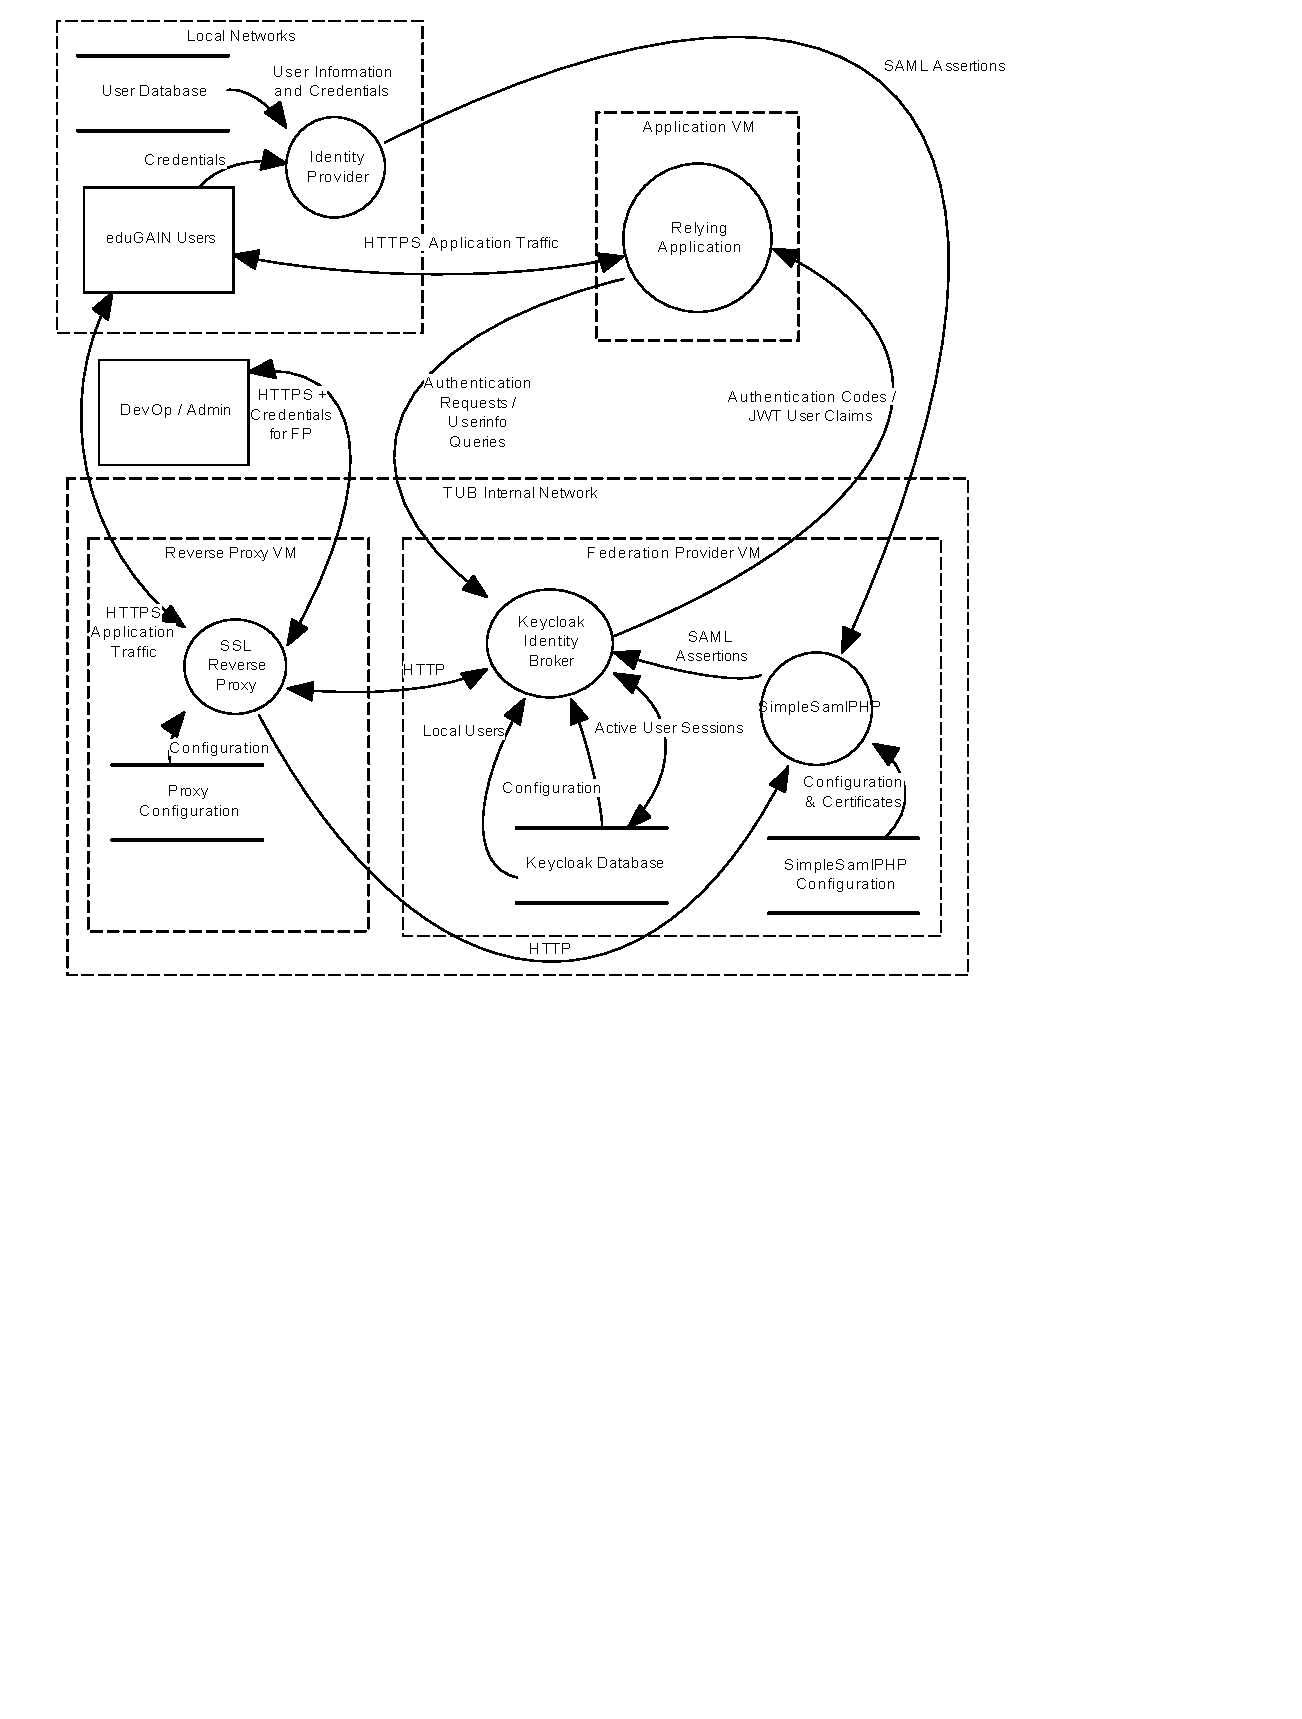
\includegraphics[width=\columnwidth, clip=true, trim=0.9cm 12.4cm 5cm 0.3cm]{data_flow}
	\caption{Federation Provider Data Flow Diagram}
	\label{fig:dataflow}
\end{figure}
	
\subsubsection{Step 4: Determining and ranking threats.}

As the last (and most important step) we compiled an extensive list of threats, their possible causes, a mitigation strategy, and the attacker type. For classifying and ranking threats we use the DREAD threat-risk model\footnote{\url{https://www.owasp.org/index.php/Application\_Threat\_Modeling\#DREAD}}. It defines the risk factors \textbf{D}amage, \textbf{R}eproducibility, \textbf{E}xploitability, \textbf{A}ffected users, and \textbf{D}iscoverability. For rating these risk factors using Low (1), Medium (2), and High(3) we relied on the Thread Rating Table\footnote{\url{https://msdn.microsoft.com/en-us/library/ff648644.aspx} (see Table 3.6)} provided by Microsoft.

At the end of the process we saw that some of the threats can be mitigated by strictly following the Open ID Connect standard and others by following industry best practice. For brevity reasons, the three top threats are:

\begin{enumerate}
	\item \textbf{Impersonation of eduGAIN users}, caused either by applications accepting JWTs without verifying them or by server impersonation to clients. This is mitigated by the design of OpenID Connect that requires applications to receive \textit{codes} which they transform into tokens, communicating directly with the Federation Provider - applications should never accept tokens from user agents. Furthermore, the connection between the applications and the Federation Provider is TLS-only, so as long as applications verify the certificate of the Federation Provider, server impersonation is prevented.
	\item \textbf{Impersonation of Federation Provider Admins} by brute-force password guessing of the Federation Provider local management accounts. To mitigate this threat, there needs to be a strong password policy, Fail2Ban\footnote{\url{http://www.fail2ban.org/}} integration, as well as potentially enforcing Keycloak two-factor authentication with time-based one-time passes\footnote{\url{https://www.youtube.com/watch?v=vHCZ6SGFT\_8}}.
	\item \textbf{Further exposure to security and privacy threats} by unintended authentication request disclosure. Those requests could contain additional data that could provoke further exposure to yet unknown threats. The OpenID standard recommends requests to always be contained in an encrypted JWT and applications to use the \texttt{request} and \texttt{request\_uri} parameters as intended\footnote{More info in Section 16.1. of \url{http://openid.net/specs/openid-connect-core-1\_0.html}}.
\end{enumerate}

\section{Extensions and Open Issues}
\label{sec:future}

This section highlights a number of future extensions and open issues associated with the security architecture.

\subsection{Automated Registration of OpenID Connect Clients}

As we've shown earlier, the security architecture enables a much more streamlined registration procedure than using eduGAIN directly. However, creating new OpenID Connect clients for each cloud application deployment is still a manual process. In order to automate the process we'll implement an API that can be used by the deployment scripts to automatically register the newly deployed applications as OpenID Connect clients. This includes the secure exchange of OpenID Client identifiers and associated secrets. According to the JWT spec the secret can be either a client-specific shared secret or a cryptographic certificate used for signing and verification.

\subsection{End-to-End Data Security in Cloud Environments}

Our previous work \cite{S13d} establishes an end-to-end data security protocol, based on TLS - the Trusted Cloud Transfer Protocol (TCTP). In \cite{SERKZ14} we have already demonstrated that it can be successfully deployed in production environments. To enable the users of the security architecture to also benefit from its additional security characteristics, we will work on integrating TCTP into the security architecture.

\subsection{Attribute-based Access Control and Secure Trust Bootstrapping}

In our past publications \cite{DLLG10,NMDL12} we showed how a distributed attribute-based access control infrastructure, such as XACML, can provide many benefits in dynamically provisioned cloud environments. In the future we will integrate this work into the security architecture to create opportunities for new use cases as well as further reduce management effort - especially when multiple cloud applications share the same access control policies.

\subsection{Open Issues}

We see two main open issues for which we don't yet have an optimal solution:

\subsubsection{Federated authentication using non-browser software.}

Both OpenID Connect as well as SAML are aimed for usage by browsers. When trying to use them with non-browser software, e.g., RESTful API clients, there are a lot of issues. For OpenID Connect there is the Direct Access Grant\footnote{\url{https://keycloak.github.io/docs/userguide/keycloak-server/html/direct-access-grants.html}} flow to directly retrieve an identity token using a username/password combination, but this has many negative security implications. For SAML2.0 there is the "Enhanced Client or Proxy"\footnote{\url{https://wiki.shibboleth.net/confluence/display/CONCEPT/ECP}} that supports SAML2.0 clients which are \textit{not} browsers. While there is a working implementation in the Shibboleth Identity Provider, not one of the 2000+ eduGAIN identity providers has enabled it.

\subsubsection{Federated access delegation to cloud resources.} While the PAM module allows people to use their federated identities for logging into systems, allowing those systems (or applications on those VMs) to access other cloud resources on behalf of the federated identity is still an ongoing issue. While there are related technologies, such as OAuth or Kerberos, we did not find a simple to use and economically feasible solution to apply.

\section{Summary and Outlook}
\label{sec:summary}

\bibliographystyle{splncs03}
\bibliography{gecon2016}

\end{document}